\part*{Week 2}
\section*{Chapter 2}
\underline{1-6, 9-13, 17, 26}
\subsection*{Problem 1}
Using atomic weights given in Table 1, calculate the molecular and equivalent weights of \\(a) alum
(\(\textnormal{Al}_2(\textnormal{SO}_4)_3\cdot 14.3\textnormal{H}_2\textnormal{O}\)), (b) lime, (c) ferrous sulfate (FeS\(\textnormal{O}_4\)\(\cdot\)7\(\textnormal{H}_2\)O), (d) fluorosilicic acid, and (e) soda ash.\\
\rule{5cm}{1pt}
\begin{description}
    \item [(a)]\[\textnormal{Atomic Weight} = 2\times 27+3\times 96+14.3\times(2+16)=\boxed{600\textnormal{ amu}}\]
    \[\textnormal{Total Valence: } 3\times 2 = 6\]
    \[\textnormal{Equivalent Weight} = \frac{600}{6}=\boxed{100\textnormal{ amu}}\]
    \item [(b)]
    \[\textnormal{Atomic Weight} =\boxed{56.1\textnormal{ amu}}\]
    \[\textnormal{Equivalent Weight} =\boxed{28\textnormal{ amu}}\]
    \item [(c)]
    \[\textnormal{Atomic Weight} =\boxed{278\textnormal{ amu}}\]
    \[\textnormal{Equivalent Weight} =\boxed{139\textnormal{ amu}}\]
    \item [(d)]
    \[\textnormal{Atomic Weight} =\boxed{144\textnormal{ amu}}\]
    \[\textnormal{Equivalent Weight} =\boxed{\textnormal{N/A}}\]
    \item [(e)]
    \[\textnormal{Atomic Weight} =\boxed{106\textnormal{ amu}}\]
    \[\textnormal{Equivalent Weight} =\boxed{53\textnormal{ amu}}\]
\end{description}
\subsection*{Problem 2}
What ions are formed when the following compounds dissolve in water: (a) sodium nitrate, (b) sulfuric acid, (c) calcium hypochlorite, and (d) sodium carbonate.\\
\rule{5cm}{1pt}
\begin{description}
    \item [(a)]
    \[\boxed{\textnormal{Na}^+\textnormal{ and NO}_3^-}\]
    \item [(b)]
    \[\boxed{\textnormal{2H}^+\textnormal{ and HSO}_4^-}\]
    \item [(c)]
    \[\boxed{\textnormal{Ca}^{++}\textnormal{ and 2OCl}^-}\]
    \item [(d)]
    \[\boxed{\textnormal{2Na}^+\textnormal{ and CO}_3^{=}}\]
\end{description}
\subsection*{Problem 3}
All of the fluoridation chemicals listed in Table 2-3 yield \(\textnormal{F}^-\) ions in solution. If 1.0 mg of fluorosilicic acid is added to water, what is the increase in concentration?\\
\rule{5cm}{1pt}
\[\textnormal{Ratio of Fluorine in Fluorosilicic Acid}=\frac{6\times 19\textnormal{ amu}}{144\textnormal{ amu}}=0.79\]
\[\textnormal{Concentration}=1\textnormal{ mg}\times 0.79=\boxed{0.79 \textnormal{ mg/L}}\]
\subsection*{Problem 4}
If a water contains 29 mg/L of \(\textnormal{Ca}^{++}\) and 16.4 mg/L of \(\textnormal{Mg}^{++}\), what is the hardness expressed in milligrams per liter as CaC\(\textnormal{O}_3\)?\\
\rule{5cm}{1pt}
\[\textnormal{Hardness of }\textnormal{Ca}^{++}\textnormal{ and Mg}^{++}=29\textnormal{ mg/L}\,\frac{\textnormal{EW CaCO}_3\textnormal{ amu}}{\textnormal{EW Ca amu}}+16.4\textnormal{ mg/L}\,\frac{\textnormal{EW CaCO}_3\textnormal{ amu}}{\textnormal{EW Mg amu}}\]
\[\textnormal{Hardness of }\textnormal{Ca}^{++}\textnormal{ and Mg}^{++}=29\textnormal{ mg/L}\,\frac{50\textnormal{ amu}}{20\textnormal{ amu}}+16.4\textnormal{ mg/L}\,\frac{50\textnormal{ amu}}{12.2\textnormal{ amu}}=\boxed{140\textnormal{ mg/L}}\]
\subsection*{Problem 5}
If a water contains 175 mg/L of calcium hardness and 40 mg/L of magnesium hardness, what are the concentrations of \(\textnormal{Ca}^{++}\) and \(\textnormal{Mg}^{++}\) ions?\\
\rule{5cm}{1pt}
\[\textnormal{Ca}^{++}=\textnormal{EW Ca amu}\,\frac{\textnormal{Ca Hardness mg/L}}{\textnormal{EW CaCO}_3\textnormal{ amu}}=20\textnormal{ amu}\,\frac{175\textnormal{ mg/L}}{50\textnormal{ amu}}=\boxed{70 \textnormal{ mg/L}}\]
\[\textnormal{Mg}^{++}=\textnormal{EW Mg amu}\,\frac{\textnormal{Mg Hardness mg/L}}{\textnormal{EW CaCO}_3\textnormal{ amu}}=12.2\textnormal{ amu}\,\frac{40\textnormal{ mg/L}}{50\textnormal{ amu}}=\boxed{9.8 \textnormal{ mg/L}}\]
\subsection*{Problem 6}
The alkalinity of a water consists of 12 mg/L of C\(\textnormal{O}_3^-\) and 100 mg/L of HC\(\textnormal{O}_3^-\). Calculate the alkalinity in milligrams per liter as CaC\(\textnormal{O}_3\).\\
\rule{5cm}{1pt}
\[\textnormal{Alkalinity }=\textnormal{mg/L CO}_3\,\frac{\textnormal{EW CaCO}_3\textnormal{ amu}}{\textnormal{EW CO}_3\textnormal{ amu}}+\textnormal{mg/L HCO}_3\,\frac{\textnormal{EW CaCO}_3\textnormal{ amu}}{\textnormal{EW HCO}_3\textnormal{ amu}}\]
\[\textnormal{Alkalinity }=12\textnormal{ mg/L}\,\frac{50\textnormal{ amu}}{30\textnormal{ amu}}+100\textnormal{ mg/L}\,\frac{50\textnormal{ amu}}{61\textnormal{ amu}}=\boxed{102\textnormal{ mg/L}}\]
\newpage
\subsection*{Problem 9}
Draw a milliequivalents-per-liter bar graph for the following water analysis:\\\\
\begin{tabular}{l l}
    C\(\textnormal{a}^{++}\) = 60 mg/L & HC\(\textnormal{O}_{3}^-\) = 115 mg/L as CaC\(\textnormal{O}_3\) \\
    M\(\textnormal{g}^{++}\) = 10 mg/L & S\(\textnormal{O}_{4}^{=}\) = 96 mg/L \\
    N\(\textnormal{a}^{+}\) = 7 mg/L  &  C\(\textnormal{l}^{-}\) = 11 mg/L \\
    \(\textnormal{K}^{+}\) = 20 mg/L &
\end{tabular}
\\\\
\rule{5cm}{1pt}
\begin{center}
\begin{tabular}{l c c c}
    Molecule & mg/L & EW & meq/L\\
    \hline
    Ca & 60 & 20 & 3\\
    Mg & 10 & 12.2 & 0.8\\
    Na & 7 & 23 & 0.3\\
    K & 20 & 39.1 & 0.5\\
    HC\(\textnormal{O}_3\) & 115 & 50 & 2.3\\
    S\(\textnormal{O}_4\) & 96 & 48 & 2\\
    Cl & 11 & 35.5 & 0.3
\end{tabular}\\
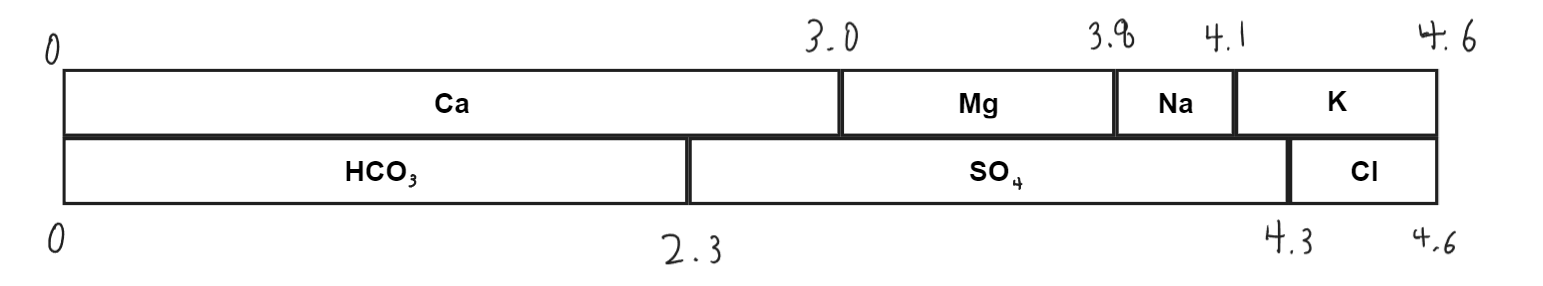
\includegraphics[scale=0.3]{diagram1.png}
\end{center}

\subsection*{Problem 10}
A brackish groundwater in an arid region has the following chemical characteristics:\\\\
\begin{tabular}{l l}
    C\(\textnormal{a}^{++}\) = 108 mg/L & HC\(\textnormal{O}_{3}^-\) = 146 mg/L \\
    M\(\textnormal{g}^{++}\) = 44 mg/L & S\(\textnormal{O}_{4}^{-2}\) = 110 mg/L \\
    N\(\textnormal{a}^{+}\) = 138 mg/L  &  C\(\textnormal{l}^{-}\) = 366 mg/L\\
\end{tabular}
\\\\
Draw the milliequivalents-per-liter bar graph. Calculate the carbonate hardness (associated with the bicarbonate ion), noncarbonated hardness, total hardness, sodium ion concentration, and alkalinity.
\\
\rule{5cm}{1pt}
\begin{center}
\begin{tabular}{l c c c}
    Molecule & mg/L & EW & meq/L\\
    \hline
    Ca & 108 & 20 & 5.4\\
    Mg & 44 & 12.2 & 3.6\\
    Na & 138 & 23 & 6\\
    HC\(\textnormal{O}_3\) & 146 & 61 & 2.4\\
    S\(\textnormal{O}_4\) & 110 & 48 & 2.3\\
    Cl & 366 & 35.5 & 10.3
\end{tabular}\\
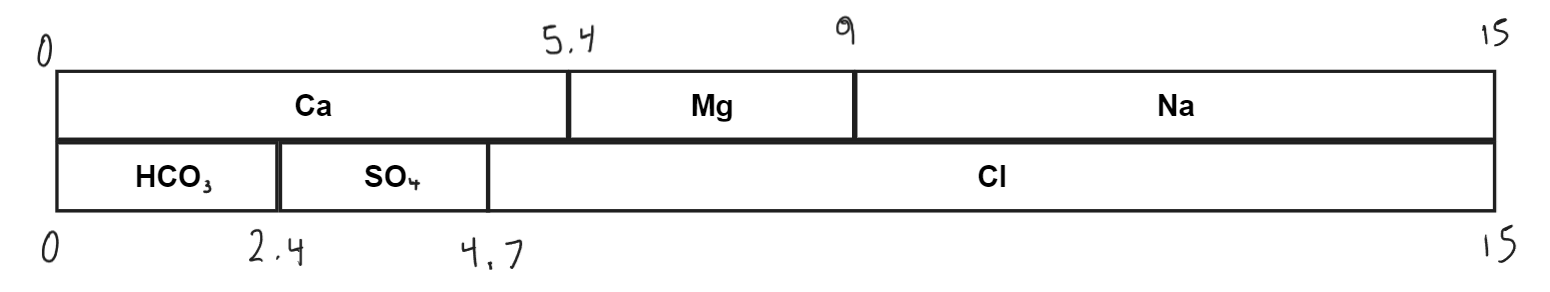
\includegraphics[scale=0.33]{diagram2.png}
\end{center}
\[\textnormal{Carbonate Hardness }=2.4\textnormal{ meq/L}\times 50\textnormal{ amu}=\boxed{120 \textnormal{ mg/L}}\]
\[\textnormal{Noncarbonate Hardness }=(5.4\textnormal{ meq/L}-2.4\textnormal{ meq/L})\times 50\textnormal{ amu}=\boxed{150 \textnormal{ mg/L}}\]
\[\textnormal{Total Hardness }=9\textnormal{ meq/L}\times 50\textnormal{ amu}=\boxed{450 \textnormal{ mg/L}}\]
\[\textnormal{Alkalinity }=2.4\textnormal{ meq/L}\times 50\textnormal{ amu}=\boxed{120 \textnormal{ mg/L}}\]
\newpage
\subsection*{Problem 11}
Draw a milliequivalents-per-liter graph and list the hypothetical combinations of chemicals in solution for the following:\\\\
\begin{tabular}{l c l}
    Calcium hardness & = & 150 mg/L \\
    Magnesium hardness & = & 65 mg/L \\
    Sodium ion & = & 8 mg/L \\
    Potassium ion & = & 4 mg/L \\
    Alkalinity & = & 190 mg/L \\
    Sulfate ion & = & 29 mg/L \\
    Chloride ion & = & 10 mg/L \\
    pH & = &  7.7
\end{tabular}
\\\\\rule{5cm}{1pt}
\begin{center}
\begin{tabular}{l c c c}
    Molecule & mg/L & EW & meq/L\\
    \hline
    Ca & 150 & 50 & 3\\
    Mg & 65 & 50 & 1.3\\
    Na & 8 & 23 & 0.3\\
    K & 4 & 39.1 & 0.1\\
    HC\(\textnormal{O}_3\) & 190 & 50 & 3.8\\
    S\(\textnormal{O}_4\) & 29 & 48 & 0.6\\
    Cl & 10 & 35.5 & 0.3
\end{tabular}\\
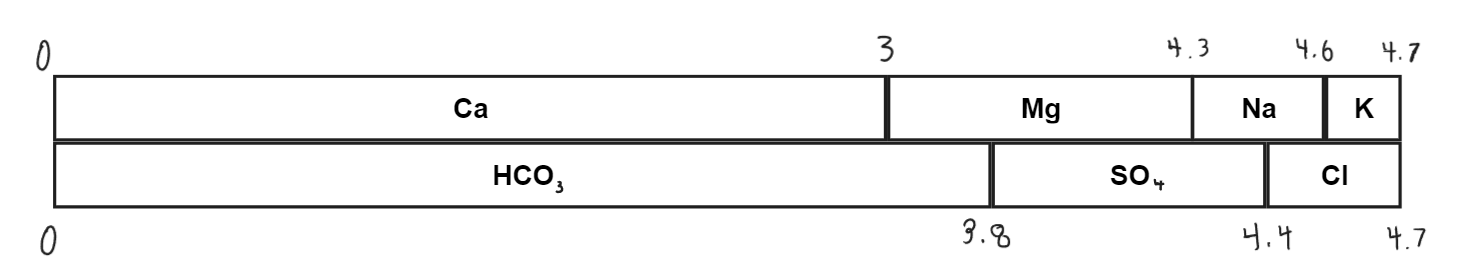
\includegraphics[scale=0.33]{diagram3.png}
\end{center}
\[\textnormal{Combinations (in meq/L): } \boxed{3 \textnormal{ Ca(HCO}_3)_2,\,0.8 \textnormal{ Mg(HCO}_3)_2,\,0.5\textnormal{ MgSO}_4,\,0.1\textnormal{ Na}_2\textnormal{SO}_4,\,0.2\textnormal{ NaCl},\,0.1\textnormal{ KCl}}\]
\subsection*{Problem 12}
A sulfuric acid solution is added to scale-forming water to convert calcium carbonate to calcium bicarbonate. Write the chemical equation for this reaction, and calculate the amount of sulfuric acid in milligrams per liter to neutralize 20 mg/L of calcium carbonate.\\
\rule{5cm}{1pt}
\[\textnormal{Balanced Reaction: }\boxed{\textnormal{H}_2\textnormal{SO}_4+2\textnormal{CaCO}_3\,\rightarrow\,\textnormal{Ca(HCO}_3)_2+\textnormal{CaSO}_4}\]
\[\textnormal{Molecular Weight CaCO}_3=100\times 2=200\textnormal{ amu}\]
\[\textnormal{Molecular Weight H}_2\textnormal{SO}_4=98.1\times 1=98.1\textnormal{ amu}\]
\[\frac{\textnormal{mg/L CaCO}_3}{\textnormal{Molecular Weight CaCO}_3}=\frac{\textnormal{mg/L H}_2\textnormal{SO}_4}{\textnormal{Molecular Weight H}_2\textnormal{SO}_4}\]
\[\frac{20\textnormal{ mg/L}}{\textnormal{200 amu}}=\frac{x \textnormal{ mg/L H}_2\textnormal{SO}_4}{98.1\textnormal{ amu}}\]
\[x=\boxed{9.81\textnormal{ mg/L}}\]
\subsection*{Problem 13}
Calculate the pH of a solution containing 10 mg/L of sulfuric acid.\\
\rule{5cm}{1pt}
\[\textnormal{Molecular Weight H}_2\textnormal{SO}_4=98.1\textnormal{ amu}\]
\[\textnormal{H}^+=\frac{1 \textnormal{ g}}{10 \textnormal{ mg}}\div 98.1\textnormal{ amu}=1.01\times 10^{-4}\textnormal{ g/L}\]
\[\textnormal{pH}=-\log(\textnormal{H}^+)=-\log(1.01\times 10^{-4})=\boxed{4}\]
\subsection*{Problem 17}
In softening of water, lime slurry Ca(OH\()_2\) is added to precipitate the calcium ion, associated with the bicarbonate radical, as CaC\(\textnormal{O}_3\). Write a balanced equation for this reaction. Calculate the amount of lime as calcium oxide necessary to react with 100 mg/L of calcium hardness.\\
\rule{5cm}{1pt}
\[\textnormal{Balanced Reaction: }\boxed{\textnormal{Ca(OH)}_2+\textnormal{Ca(HCO}_3\textnormal{)}_2\,\rightarrow\,2\textnormal{CaCO}_3+2\textnormal{H}_2\textnormal{O}}\]
\[\frac{\textnormal{EW CaO amu}}{\textnormal{EW CaCO}_3\textnormal{ amu}}=\frac{x\textnormal{ mg/L CaO}}{\textnormal{mg/L CaCO}_3}\]
\[\frac{28\textnormal{ amu}}{50\textnormal{ amu}}=\frac{x\textnormal{ mg/L CaO}}{100\textnormal{ mg/L}}\]
\[x=\boxed{56\textnormal{ mg/L}}\]
\subsection*{Problem 26}
In Eq. 29, why is the value of the constant 50,000 to calculate alkalinity as CaC\(\textnormal{O}_3\)?\\
\rule{5cm}{1pt}
\[\textnormal{Alkalinity }=\frac{\textnormal{mL Titrant}\times\textnormal{Normality of Acid}\times x}{\textnormal{mL Sample}}\]
Where, according to the textbook, the volume of the titrant is 1 mL, the volume of the sample is 100 mL, the alkalinity is 10 mg/L, and the normality of the acid is 0.02 N.
\[\textnormal{10 mg/L}=\frac{1\textnormal{ mL}\times 0.02\textnormal{ N}\times x}{\textnormal{100 mL}}\]
\[x=\frac{\textnormal{10 mg/L}\times\textnormal{100 mL}}{1\textnormal{ mL}\times 0.02\textnormal{ N}}=\boxed{50000}\]